%\documentclass[envcountsect,11pt,trans]{beamer}
\documentclass[11pt,aspectratio=169]{beamer}
\usepackage[english]{babel}
\usepackage[ansinew]{inputenc}
\usepackage{times}
\usepackage{xcolor}
\usepackage{graphicx}
\usepackage{rotating}
\usepackage{bbding,pifont} % two dingbat fonts
\usepackage{amsmath}
\usepackage{amsfonts}
\usepackage{amssymb}
\usepackage{fancybox}
\usepackage{epstopdf}
\usepackage{eso-pic}
%\usepackage[round]{natbib}
\usepackage{ngerman}
\usepackage{tcolorbox}
\usepackage{colortbl}
%\usepackage[authordate,bibencoding=auto,strict,backend=biber]{biblatex-chicago}
%\usepackage{natbib}
%\usepackage[style=bath, backend=biber]{biblatex}
\usepackage{ulem}
\usepackage{tikz}
\usepackage{booktabs}
\usepackage{longtable}
\usepackage{hyperref}
\usepackage{array}
\usepackage{appendixnumberbeamer}
\usepackage[T1]{fontenc}
\usepackage{adjustbox}
\usepackage{listings}
\usepackage{uarial}
\usepackage{fancyvrb}
\usepackage{subfigure}
\renewcommand{\familydefault}{\sfdefault}

\newcommand*\circled[1]{\tikz[baseline=(char.base)]{
            \node[shape=circle,draw,inner sep=2pt] (char) {#1};}}
\newcommand{\E}{\operatorname{E}}
\newcommand{\Var}{\operatorname{Var}}
\newcommand{\overbar}[1]{\mkern 1.5mu\overline{\mkern-1.5mu#1\mkern-1.5mu}\mkern 1.5mu}
\DeclareMathOperator*{\argmin}{arg\,min}
\DeclareMathOperator*{\argmax}{arg\,max}
% \use\smallpackage{pgfpages}
% \pgfpagesuselayout{4 on 1}[a4paper,border shrink=10mm,landscape]

%\xdefinecolor{MyColor}{rgb}{0.14,0.17,0.52}
%\xdefinecolor{MyColor}{rgb}{0.29,0.53,0.82}
%\xdefinecolor{MyBlue}{rgb}{0.14,0.17,0.52}
%\xdefinecolor{MyGreen}{rgb}{0.70,0.78,0.14}
%\xdefinecolor{MyAlert}{rgb}{0.29,0.53,0.82}
%\colorlet{mystructure}{MyColor}
%\usecolortheme[named=mystructure]{structure}
%\setbeamercolor{alerted text}{fg=MyAlert}
\definecolor{Black}{RGB}{0,0,0}
\definecolor{RedGIZ}{RGB}{200,15,15}
\setbeamercolor{title}{fg=black}
\setbeamercolor{section in toc}{fg=black}
\setbeamercolor{subsection in toc}{fg=black}
\setbeamercolor{frametitle}{fg=Black}
\setbeamercolor{tableofcontents}{fg=Black}

%\usetheme{Boadilla}
%\usetheme{Madrid}
%\useoutertheme{infolines}
%\usecolortheme{whale}
%\usecolortheme{lily}
\renewcommand{\inserttitlegraphic}{
\parbox[b][2.5cm][t]{4cm}{
\includegraphics[width = 4cm, keepaspectratio]{pictures/GIZ_Logo.png}}  \hspace{0.1cm} \parbox[b][2.5cm][t]{4cm}{
\includegraphics[width = 4cm, keepaspectratio]{pictures/IWH_Logo_RGB_DE_Grossformat.png}} \hfill \parbox[b][2.5cm][t]{3.21cm}{
\includegraphics[keepaspectratio,width=4.00cm]{pictures/seperationbar.png} \\ \includegraphics[width = 4cm, keepaspectratio]{pictures/BMWI_logo.png}}
}
\defbeamertemplate*{title page}{customized}[1][]
{	
	\vspace{2.75cm}
  \usebeamerfont{title}\begin{center}\textbf{\inserttitle}\end{center}\par
  \usebeamerfont{subtitle}\begin{center}\usebeamercolor[fg]{subtitle}\insertsubtitle\end{center}\par
  \usebeamerfont{author}\insertauthor $\, \vert$ \usebeamerfont{date}\insertdate \par
  \usebeamerfont{institute}\insertinstitute\par
	\vspace{0.25cm}
  \usebeamercolor[fg]{titlegraphic}\inserttitlegraphic


}
\setbeamerfont{subtitle}{size=\normalsize}
\setbeamerfont{author}{size=\tiny}
\setbeamerfont{date}{size=\tiny}
\setbeamerfont{institute}{size=\tiny}

\setbeamercovered{transparent}

\setbeamertemplate{footline}[text line]{%
  \parbox{\linewidth}{\vspace*{-8pt} $\vert$ \hspace{1mm} \today \hspace{1mm} $\vert$ \hfill}}
\setbeamertemplate{navigation symbols}{}

\linespread{1.2}





\mode<presentation>{
    \setbeamertemplate{itemize item}{\color{RedGIZ}$\blacksquare$}
    \setbeamertemplate{itemize subitem}{\color{RedGIZ}$\blacktriangleright$}
		}
\title[DGE-CRED]{Dynamic General Equilibrium Model for Climate Resilient Economic Development}
%\subtitle[]{Training}

\author[Christoph Schult]{Andrej Drygalla and Christoph Schult} \date[June 2020]{June 2020}

\institute[IWH]{Halle Institute for Economic Research}

 
\logo{\begin{tabular}{c}
\includegraphics[keepaspectratio,width=1.00cm]{pictures/seperationbar.png} \\ 
\includegraphics[keepaspectratio,width=1.00cm]{pictures/GIZ_Logo}\end{tabular}}

\usepackage[style=authoryear-comp,maxbibnames=9,maxcitenames=2,backend=bibtex]{biblatex}
\bibliography{references}

% Settings by yw:
% Outline at beginning of each section:
\AtBeginSection[] {
	\begin{frame}<beamer>{Outline}
		\tableofcontents[sectionstyle=show/hide, subsectionstyle=show/show/hide, subsubsectionstyle=show/show/hide]
	\end{frame}
}
% Packages:
\usepackage{subfigure}
\usepackage{ragged2e}
% Section numbering:
\setbeamertemplate{section in toc}[sections numbered]
\setbeamertemplate{subsection in toc}[subsections numbered]
\setbeamertemplate{subsubsection in toc}[subsubsections numbered]
\setbeamertemplate{section in toc}[ball]
\setbeamertemplate{subsection in toc}[ball]
\setbeamertemplate{subsubsection in toc}[ball]
\setbeamercolor{section number projected}{bg={RedGIZ}}
\setbeamercolor{subsection number projected}{bg={RedGIZ}}
\setbeamercolor{subsubsection number projected}{bg={RedGIZ}}

\begin{document}
%\footnotesize
\usebackgroundtemplate{
\vbox to \paperheight{\vspace{0.1cm}\hbox to \paperwidth{\hfil
\includegraphics[width=0.975\paperwidth,height = 0.7\paperheight]{pictures/BackgroundGIZ.jpg}\hfil}\vfil
}}

\begin{frame}<presentation>[noframenumbering,plain]
  \titlepage
\end{frame}
\usebackgroundtemplate{
}
\begin{frame}<presentation>[noframenumbering]
	\frametitle{Outline}
		 \tableofcontents[hideallsubsections]
\end{frame}

\section{Introduction to Dynare}

\subsection{What is Dynare?}
\begin{frame}<presentation>
\frametitle{{\thesection.\thesubsection} What is Dynare?}
  \begin{itemize}
		\item Dynare is an open-source program for dynamic general equilibrium modeling,
		\item mainly a collection of different functions written for Matlab,
		\item preprocessor translates mod files into matlab code.
	\end{itemize}
\end{frame}

\subsection{Neoclassical Growth Model}
\begin{frame}<presentation>
\frametitle{{\thesection.\thesubsection} Neoclassical Growth Model (1)}
	 \begin{itemize}
	 	\item In order to illustrate the basic structure of Dynare, this section considers the following neoclassical growth model:
	 	\begin{gather*}
	 	\underset{\left\{ c_t, k_t\right\} _{t=1}^{\infty}}{\max} = \sum_{t=1}^{\infty} \beta^{t-1} \frac{c_t^{1-\sigma}}{1-\sigma}\\
	 	\text{s.t.} \quad c_t + k_t = A_t k_{t-1}^{\alpha} + (1-\delta) k_{t-1}
	 	\end{gather*}
	 	\item The resulting first order conditions are:
	 	\begin{gather*}
	 	c_t^{-\sigma} = \beta c_{t+1}^{-\sigma} (\alpha A_{t+1} k_t^{\alpha -1} + 1 - \delta)\\
	 	c_t + k_t = A_t k_{t-1}^\alpha + (1-\delta) k_{t-1}
	 	\end{gather*}
	\end{itemize}
\end{frame}
\begin{frame}<presentation>
	\frametitle{{\thesection.\thesubsection} Neoclassical Growth Model (2)}
	\begin{itemize}
		\justifying
		\item The steady state can be obtained analytically and is characterized by the following two equations:
		\begin{gather*}
		\bar{k} = \bigg(\frac{1-\beta (1-\delta)}{\beta\alpha\bar{A}}\bigg)^\frac{1}{\alpha -1}\\
		\bar{c} = \bar{A} \bar{k}^\alpha - \delta \bar{k}		
		\end{gather*}
		\item The neoclassical growth model considered in these slides, as well as the DGE-CRED model are deterministic models. There are no stochastic elements requiring expectancy terms or probability distributions. Therefore, the remained of this introduction to Dynare focuses on this class of models.
	\end{itemize}
\end{frame}

\subsection{Setting up a Model File}
\begin{frame}<beamer>{Outline}
	\tableofcontents[sectionstyle=hide/hide, subsectionstyle=show/shaded/hide, subsubsectionstyle=show/show/hide]
\end{frame}
\subsubsection{Model File}
\begin{frame}<presentation>[fragile]
	\frametitle{{\thesection.\thesubsection.\thesubsubsection} Model File}
	\begin{itemize}
		\justifying
		\item A model file (filename.mod) contains commands and blocks. Each command and each element of a block is terminated by a semicolon (;). Blocks are terminated by \texttt{end;} .
		\item The model file used for this introduction to Dynare is entername.mod and it is recommendable to take a look at that file while proceeding with these slides. 
		\item Code lines within the mode file can be enabled using \%, // or /* ... */.
		\item In order to run a model file (i) the Dynare path has to be added to the search path of MATLAB and (ii) Dynare executed to run the model in MATLAB:
			\begin{verbatim}
				   addpath('C:\dynare\4.6.1\matlab')
				   dynare filename
			\end{verbatim}
	\end{itemize}
\end{frame}
\subsubsection{Variables and Parameters}
\begin{frame}<presentation>[fragile]
	\frametitle{{\thesection.\thesubsection.\thesubsubsection} Variables and Parameters (1)}
	\begin{itemize}
		\justifying
		\item At the beginning of each model file, the endogenous (\texttt{var}) and exogenous (\texttt{varexo}) variables as well as parameters (\texttt{parameters}) have to be defined:
			\begin{verbatim}
			   var = c k;		
			   varexo = A;		
			   parameters alpha_p beta_p gamma_p delta_p;	
			\end{verbatim}	
		\item Then, the parameter values have to be assigned:
			\begin{verbatim}				
			   alpha_p = 0.5;
			   beta_p = 0.95;
			   gamma_p = 0.5;
			   delta_p = 0.02;
			\end{verbatim}
	\end{itemize}
\end{frame}
\begin{frame}<presentation>[fragile]
	\frametitle{{\thesection.\thesubsection.\thesubsubsection} Variables and Parameters (2)}
	\begin{itemize}
		\item Optionally, a LaTeX name and long name can be assigned to a variable using the convention:\\ \texttt{variable\_name \$tex\_name\$ (long\_name = 'quoted\_string')}.
		\begin{verbatim}
		  var 
		  k $k$ (long_name = 'capital'),
		  c $c$ (long_name = 'consumption'),
		  ;
		  varexo 
		  A $A$ (long_name = 'technology'),
		  ;
		\end{verbatim}
	\end{itemize}
\end{frame}
\begin{frame}<presentation>
	\frametitle{{\thesection.\thesubsection.\thesubsubsection} Variables and Parameters (3)}
	\begin{itemize}
		\justifying
		\item There are some restrictions to kept in mind, when choosing variable and parameter names in Dynare. First, variables and parameters must not have the same name as Dynare commands or build-in functions. Second, minimize interference with MATLAB or Octave functions. In particular, do not use correctly-spelled greek letters like \texttt{beta}, because there are MATLAB functions of the same name.
		\item Note that by convention in Dynare, the time indice of a variable reflects when this variable is decided. The typical example is for capital stock: since the capital stock entering the production function in the current period is decided in the previous period, the capital stock becomes \texttt{k(-1)}, and the law of motion of capital must be written: \texttt{k = i + (1-delta)*k(-1)}.\footnote{This convention can be modified using the \texttt{predetermined\_variables} setting.} 
	\end{itemize}
\end{frame}
\subsubsection{The \texttt{model} block}
\begin{frame}<presentation>[fragile]
	\frametitle{{\thesection.\thesubsection.\thesubsubsection} The \texttt{model} block}
	\begin{itemize}
		\justifying
		\item A model is declared inside a \texttt{model} block. In general, there must be as many equations as there are endogenous variables in the model. A great advantage of using Dynare is that the equations can be written almost as on paper.
		\begin{verbatim}
		   model;
		   c + k = A*k(-1)^alpha_p + (1-delta_p)*k(-1);
		   c^(-gamma_p) = beta_p*c(+1)^(-gamma_p)
		           *(alpha_p*A(+1)*k^(alpha_p-1) + 1 - delta_p);
		   end;
		\end{verbatim}
		\item Now, the model is set up and one can begin with the deterministic simulation. 
	\end{itemize}
\end{frame}

\subsection{Deterministic Simulation}
\begin{frame}<presentation>[fragile]
	\frametitle{{\thesection.\thesubsection} Deterministic Simulations in Dynare (1)}
	\begin{itemize}
		\justifying
		\item The deterministic simulation builds up on the concept of perfect foresight, in which agents have full knowledge and perfectly anticipate all future shocks.
		\item Concretly, at period 1:
		\begin{itemize}
			\item agents learn the value of all future shocks;
			\item since there is shared knowledge of the model and of future shocks, agents can compute their optimal plans for all future periods;
			\item optimal plans are not adjusted in periods 2 and later\\ $\Rightarrow$ the model behaves as if it were deterministic.
		\end{itemize}
		\item Cost of this approach: the effect of future uncertainty is not taken into account.
		\item Advantage: numerical solutions can be computed exactly (up to rounding errors) and nonlinearities are fully taken into account.
	\end{itemize}
\end{frame}
\begin{frame}<presentation>
	\frametitle{{\thesection.\thesubsection} Deterministic Simulations in Dynare (2)}
	\begin{itemize}
		\item The general problem in the deterministic, perfect foresight, case can be expressed as: $$f(y_{t+1},y_t,y_{t-1},u_t)=0,$$ where $y$ is the vector of endogenous variables and $u$ the vector of exogenous shocks.
		\item Identification rule: there must be as many equations in $f(...)$ as there are endogneous variables in $y$.
	\end{itemize}
\end{frame}
\begin{frame}<presentation>
	\frametitle{{\thesection.\thesubsection} Deterministic Simulations in Dynare (3)}
	\begin{itemize}
		\item Accordingly, the general perfect foresight problem for the neoclassical growth model is:
		\begin{gather*}
			y_t = \begin{pmatrix} c_t \\ k_t \end{pmatrix} \\
			u_t = A_t \\
			f(y_{t+1},y_t,y_{t-1},u_t) = \begin{pmatrix} 	c_t^{-\sigma} - \beta c_{t+1}^{-\sigma} (\alpha A_{t+1} k_t^{\alpha -1} + 1 - \delta)\\ c_t + k_t - A_t k_{t-1}^\alpha - (1-\delta) k_{t-1} \end{pmatrix}
		\end{gather*}
	\end{itemize}
\end{frame}
\begin{frame}<presentation>
	\frametitle{{\thesection.\thesubsection} Deterministic Simulations in Dynare (4)}
	\begin{itemize}
		\item The aim of a deterministic simulation is to examine the trajectories of the model variables over time $t = 1,...,T$. 
		\item Consequently, the stacked system for a perfect foresight simulation over $T$ periods becomes a two-boundary value problem: 
		$$\left\{ \begin{matrix} f(y_2,y_1,\mathbin{\textcolor{red}{y_0}},\mathbin{\textcolor{blue}{u_1}})=0 \\ 
		f(y_3,y_2,y_1,\mathbin{\textcolor{blue}{u_2}})=0 \\ 
		\vdots \\ 
		f(\mathbin{\textcolor{red}{y_{T+1}}},y_T,y_{T-1},\mathbin{\textcolor{blue}{u_T}})=0 
		\end{matrix},  \right.$$ 
		where $y_0$ and $y_{T+1}$ as well as $u_1,...,u_T$ are given.
		\item Dynare uses a Newton-type methode to solve this stacked system.
	\end{itemize}
\end{frame}
\begin{frame}<presentation>
	\frametitle{{\thesection.\thesubsection} Deterministic Simulations in Dynare (5)}
	\begin{itemize}
		\justifying
		\item The previously described technique numerically computes trajectories for given shocks over a \textit{finite} number of periods. 
		\item If one is rather interested in solving an infinite-horizon problem, the easiest way is to approximate the solution by a finite-horizon problem (large $T$). The drawback of this approach is that the solution is specific to a given sequence of shocks, and not generic.  
		\item In case there is more than one lead or lag, Dynare automatically transforms the model in the form with one lead and one lag using auxiliary variables. For example, if there is a variable with two leads $x_{t+2}$:
		\begin{itemize}
			\item create a new auxiliary variable $a$
			\item replace all occurrences of $x_{t+2}$ by $a_{t+1}$
			\item add a new equation: $a_t = x_{t+1}$		
		\end{itemize}
	\end{itemize}
\end{frame}

\subsection{Perfect Foresight Setup}
\begin{frame}<beamer>{Outline}
	\tableofcontents[sectionstyle=hide/hide, subsectionstyle=show/shaded/hide, subsubsectionstyle=show/show/hide]
\end{frame}
\subsubsection{Getting stated with perfect foresight}
\begin{frame}<presentation>[fragile]
	\frametitle{{\thesection.\thesubsection.\thesubsubsection} Getting stated with perfect foresight}
	\begin{itemize}
		\justifying
		\item In order to perform the deterministic simulation, one has specify (i) the constraints of the stacked system $y_0$, $y_{T+1}$ and $u_1, \ldots , u_T$ and (ii) provide an initial guess $y_1, \ldots , y_T$ for the Newton algorithm. 
		\item The path for the endogenous and exogenous variables are stored in two MATLAB/Octave matrices:
		\begin{itemize}
			\item \texttt{oo\_.endo\_simul = ($y_0$  $y_1$ \ldots  $y_T$  $y_{T+1}$)}
			\item \texttt{oo\_.exo\_simul' = ($y_0$  $y_1$ \ldots  $y_T$  $y_{T+1}$)}
		\end{itemize}
		\item The \texttt{perfect\_foresight\_setup} initializes those matrices, given the \texttt{shocks}, \texttt{initval}, \texttt{endval} and \texttt{histval} blocks.
		\item Then, the \texttt{perfect\_foresight\_solver} replaces $y_1,\ldots,y_T$ by the solution. 
	\end{itemize}
\end{frame}
\subsubsection{The \texttt{initval} block}
\begin{frame}<presentation>
	\frametitle{{\thesection.\thesubsection.\thesubsubsection} The \texttt{initval} block (1)}
	\begin{itemize}
		\justifying
		\item In presence of the \texttt{initval} and absence of other blocks, both the \texttt{oo\_.endo\_simul} and \texttt{oo\_.exo\_simul} variables storing the endogenous and exogenous variables will be filled with the values provided by this block. If there are no other blocks present, it will therefore provide the initial and terminal conditions for all the endogenous and exogenous variables, because it will also fill the last column/row of these matrices.  For the intermediate simulation periods it thereby provides the starting values for the solver. 
		\item It is important to be aware that if some variables, endogenous or exogenous, are not mentioned in the \texttt{initval} block, a zero value is assumed.
	\end{itemize}
\end{frame}
\begin{frame}<presentation>[fragile]
	\frametitle{{\thesection.\thesubsection.\thesubsubsection} The \texttt{initval} block (2)}
	\begin{itemize}
		\justifying
		\item Example: Let us assume that we want to set $c_0=c_{T+1}=4$ and $k_0=k_{T+1}=20$ in the neocalssical growth model. Furthermore, we assume that TFP is constant at $A_t=1$. 
			\begin{verbatim}
				   initval;
				   c = 4;
				   k = 20;
				   A = 1;
				   end;
			\end{verbatim}
		\item In order to run the deterministic simulation for $T=100$ periods, enter:
			\begin{verbatim}
			   perfect_foresight_setup(periods=100);
			   perfect_foresight_solver;
			\end{verbatim}
	\end{itemize}
\end{frame}
\begin{frame}<presentation>[fragile]
	\frametitle{{\thesection.\thesubsection.\thesubsubsection} The \texttt{initval} block (3)}
	\begin{itemize}
		\item The following trajectories are obtained:
		\begin{figure}
			\centering
			\subfigure{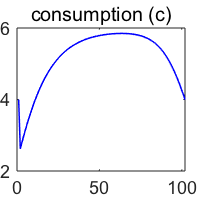
\includegraphics[width=3.5cm]{pictures/consumption01}}\qquad
			\subfigure{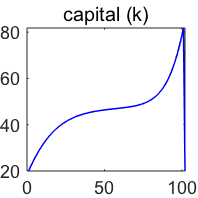
\includegraphics[width=3.5cm]{pictures/capital01}}\qquad
			\subfigure{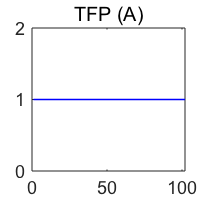
\includegraphics[width=3.5cm]{pictures/TFP01}}
		\end{figure}
		\item Comments:
			\begin{itemize}
				\item As consumption is a forward looking variable in this model, its initialization $c_0$ does not affect the trajectory. However, its terminal value does.
				\item The opposite holds for capital. 
			\end{itemize}
	\end{itemize}
\end{frame}
\subsubsection{The \texttt{endval} block}
\begin{frame}<presentation>[fragile]
	\frametitle{{\thesection.\thesubsection.\thesubsubsection} The \texttt{endval} block (1)}
	\begin{itemize}
		\justifying
		\item In the absence of an \texttt{initval} block, the \texttt{endval} block fills both \texttt{oo\_.endo\_simul} and \texttt{oo\_.exo\_simul}. In this case it, therefore, has the same effect as if only an \texttt{initval} block was present.
		\item However, if an \texttt{initval} and  \texttt{endval} block are both present, the former assigns the initial conditions in $t=0$ while the latter provides the terminal conditions in $t=T+1$ as well as the initial guess for the perfect foresight solver.
		\item Example: Let us assume that we want to set $c_0=4$, $c_{T+1}=6$, $k_0=20$, $k_{T+1}=30$ and $A_t=1$.
	\end{itemize}
\end{frame}
\begin{frame}<presentation>[fragile]
	\frametitle{{\thesection.\thesubsection.\thesubsubsection} The \texttt{endval} block (2)}
	\begin{itemize}
		\item Leading the following code:
			\begin{verbatim}
			   initval;
			   c = 4;
			   k = 20;
			   A = 1;
			   end;

			   endval;
			   c = 6;
			   k = 30;
			   A = 1;
			   end;
			\end{verbatim}
	\end{itemize}
\end{frame}
\begin{frame}<presentation>[fragile]
	\frametitle{{\thesection.\thesubsection.\thesubsubsection} The \texttt{endval} block (3)}
		\begin{itemize}
		\item The following trajectories are obtained:
		\begin{figure}
			\centering
			\subfigure{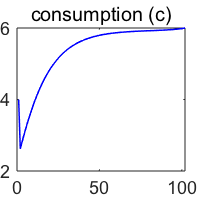
\includegraphics[width=3.5cm]{pictures/consumption02}}\qquad
			\subfigure{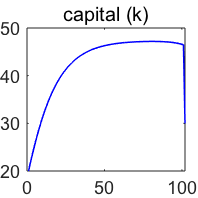
\includegraphics[width=3.5cm]{pictures/capital02}}\qquad
			\subfigure{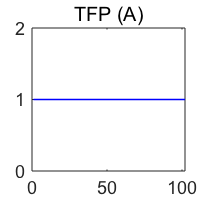
\includegraphics[width=3.5cm]{pictures/TFP02}}
		\end{figure}
		\item Comment: As in the previous example, consumption is forward looking, while capital is backward looking.
	\end{itemize}
\end{frame}
\subsubsection{The \texttt{histval} block}
\begin{frame}<presentation>[fragile]
	\frametitle{{\thesection.\thesubsection.\thesubsubsection} The \texttt{histval} block (1)}
	\begin{itemize}
		\justifying
		\item The usage of the \texttt{histval} block is particularly interesting, if there are variables with more than one lead or lag. 
		\item In a determinsitic simulation the \texttt{histval} block must be combined with an \texttt{initval} block. A \texttt{histval} and \texttt{endval} block cannot be combined.
		\item The \texttt{histval} block assigns the initial condition, while the \texttt{initval} block provides the terminal condition and inital guess for the perfect foresight solver.
	\end{itemize}
\end{frame}
\begin{frame}<presentation>[fragile]
	\frametitle{{\thesection.\thesubsection.\thesubsubsection} The \texttt{histval} block (2)}
	\begin{itemize}
		\justifying
		\item The previous example can, therefore, also be implemented by:
			\begin{verbatim}
				histval;
				c(0) = 4;
				k(0) = 20;
				A(0) = 1;
				end;
				
				initval;
				c = 6;
				k = 30;
				A = 1;
				end;
			\end{verbatim}
	\end{itemize}
\end{frame}
\subsubsection{Shocks on exogenous variables}
\begin{frame}<presentation>[fragile]
	\frametitle{{\thesection.\thesubsection.\thesubsubsection} Shocks on exogenous variables (1)}
	\begin{itemize}
		\item For deterministic simulations, the \texttt{shocks} block specifies temporary changes in the value of exogenous variables. For permanent shocks, use an \texttt{endval} block.
		\item It is possible to specify shocks which last several periods and which can vary over time.  The \texttt{periods} keyword accepts a list of several dates or date ranges, which must be matched by as many shock values in the \texttt{values} keyword. 
		\item Note that a range in the \texttt{periods} keyword can be matched by only one value in the \texttt{values} keyword.  If values represents a scalar, the same value applies to the whole range.  If values represents a vector, it must have as many elements as there are periods in the range.
	\end{itemize}
\end{frame}
\begin{frame}<presentation>[fragile]
	\frametitle{{\thesection.\thesubsection.\thesubsubsection} Shocks on exogenous variables (2)}
	\begin{itemize}
		\item The \texttt{shock} block has the following structure:
			\begin{verbatim}
			   shocks;
			   var ... ;
			   periods ... ;
			   values ... ;
			   end;
			\end{verbatim}
		\item Examples using the \texttt{shock} block will be examined at the end of this section.
	\end{itemize}
\end{frame}

\subsection{Steady State}
\begin{frame}<presentation>
	\frametitle{{\thesection.\thesubsection} Steady State}
	\begin{itemize}
		\item A steady state, $\bar{y}$, for the model satisfies: $$f(\bar{y},\bar{y},\bar{y},\bar{u})=0.$$ 
		\item Note that a steady state is conditional to:
		\begin{itemize}
			\item The steady state values of exogenous variables $\bar{u}$.
			\item The values of parameters (implicit in the above definition).
		\end{itemize}
		\item Even for a given set of exogenous and parameter values, some (nonlinear) models have several steady states.
		\item There are three approaches in Dynare to calculate the steady state.
		\item The steady state values are stored in the MATLAB/Octave matrix \texttt{oo\_.steady\_state}.
	\end{itemize}
\end{frame}
\begin{frame}<presentation>[fragile]
	\frametitle{{\thesection.\thesubsection} Steady State: Approach 1}
	\begin{itemize}
		\justifying
		\item Idea: Provide an initial guess for the steady state in the \texttt{initval} block and then conduct the steady state calculation using \texttt{steady}.
			\begin{verbatim}
				   initval;
				   ...
				   end;
				   steady;
			\end{verbatim}
		\item The obtained steady state values are then written into \texttt{oo\_.endo\_simul} and \texttt{oo\_.exo\_simul}, unless instructed otherwise. An \texttt{initval} block followed by \texttt{stedy}, therefore, has the same effect as an \texttt{initval} block containing the steady state values.
	\end{itemize}
\end{frame}
\begin{frame}<presentation>[fragile]
	\frametitle{{\thesection.\thesubsection} Steady State: Approach 2}
	\begin{itemize}
		\item Idea: Use a \texttt{steady\_state\_model} block, in which the steady state values are calculated. 
		\begin{verbatim}
		   steady_state_model;
		   ...
		   end;
		\end{verbatim}
		\item The obtained steady state values are then written into \texttt{oo\_.endo\_simul} and \texttt{oo\_.exo\_simul}, unless instructed otherwise. 
		\item In cases where the steady state can be solved analytically, using a \texttt{steady\_state\_model} block is a suitable approach. 
	\end{itemize}
\end{frame}
\begin{frame}<presentation>[fragile]
	\frametitle{{\thesection.\thesubsection} Steady State: Approach 3}
	\begin{itemize}
		\justifying
		\item  Idea: Use an explicit steady state file, which is an external MATLAB-file that must conform with a certain structure and naming convention:\\ \texttt{NAMEofMODfile\_steadystate.m}. 
		\item In this steady state file, you must provide the exact steady state values as in the case of the \texttt{steady\_state\_model} block.
		\item Advantage: flexibility, can call build-in MATLAB functions, allows for changing parameters to take parameter dependencies into account without resorting to model-local variables.
		\item Drawback: the additional flexibility offered by a steady state file increases the scope for errors.
		\item Note: A steady state file is used in the DGE-CRED model.
	\end{itemize}
\end{frame}
\subsection{Remarks}
\begin{frame}<presentation>[fragile]
	\frametitle{{\thesection.\thesubsection} Remarks on the usage of perfect foresight}
	\begin{itemize}
		\justifying
		\item  Because of the various functions of the \texttt{initval}, \texttt{endval} and \texttt{histval} blocks, it is stronglyrecommended to check the constructed \texttt{oo\_.endo\_simul} and \texttt{oo\_.exo\_simul} variables after running \texttt{perfect\_foresight\_setup} and before running \texttt{perfect\_foresight\_solver} to see whether the desired outcome has been achieved.
		\item Instead of using \texttt{perfect\_foresight\_setup} and \texttt{perfect\_foresight\_solver}, the command \texttt{simul(periods = T}) can also be used.
		\item The following slides cover some examples based on the neoclassical growth model. It is recommendable to take a look at the file entername.mod while proceeding with these examples.
	\end{itemize}
\end{frame}

\subsection{Examples}
\begin{frame}<presentation>[fragile]
	\frametitle{{\thesection.\thesubsection} Example No. 1}
	\begin{itemize}
		\item Scenario 1: Return to equilibrium starting from $k_0=0.5\bar{k}$.
			\begin{verbatim}
			   ...
			   steady;
			   
			   ik = varlist_indices('k',M_.endo_names);
			   kstar = 00_.steady_state(ik);
			   
			   histval;
			   k(0) = kstar/2;
			   end;
			   ...
			\end{verbatim}
	\end{itemize}
\end{frame}
\begin{frame}<presentation>[fragile]
	\frametitle{{\thesection.\thesubsection} Example No. 2}
	\begin{itemize}
		\item Scenario 2: The economy starts from the steady state. There is an unexpected positive productivity shock at the beginning of period 1: $A_1 = 1.1$.
		\begin{verbatim}
		   ...
		   steady;
		
		   shocks;
		   var A;
		   periods 1;
		   values 1.1;
		   end;
		   ...
		\end{verbatim}
	\end{itemize}
\end{frame}
\begin{frame}<presentation>[fragile]
	\frametitle{{\thesection.\thesubsection} Example No. 3}
	\begin{itemize}
		\justifying
		\item Scenario 3: The economy starts from the steady state. There is a sequence of shocks to $A_t$: 10\% in period 5 and an additional 5\% during the 4 following periods.
		\begin{verbatim}
	  	...
		   steady;
		
		   shocks;
		   var A;
		   periods 4, 5:8;
		   values 1.1, 1.05;
		   end;
		   ...
		\end{verbatim}
	\end{itemize}
\end{frame}
\begin{frame}<presentation>[fragile]
	\frametitle{{\thesection.\thesubsection} Example No. 4}
	\begin{itemize}
		\item Scenario 4: The economy starts from the initial steady state. In period 1, TFP increases by 10\% permanently.
		\begin{verbatim}
		   ...
		   initval;
		   A = 1;
		   end; 
		   steady;
		
		   endval;
		   A = 1.1;
		   end;
		   steady;
		   ...
		\end{verbatim}
	\end{itemize}
\end{frame}
\begin{frame}<presentation>[fragile]
	\frametitle{{\thesection.\thesubsection} Example No. 5}
	\begin{itemize}
		\item Scenario 5: The economy starts from the initial steady state. In period 6, TFP increases by 10\% permanently. 
			\begin{itemize}
				\item Same \texttt{initval} and \texttt{endval} blocks as in Scenario 4.
				\item A shock block is used to maintain TFP at its initial level during periods 1-5.
			\end{itemize}
		\begin{verbatim}
		   ...
		   shocks;
		   var A;
		   periods 1:5;
		   values 1;
		   end;
		   ...
		\end{verbatim}
	\end{itemize}
\end{frame}

\subsection{Newton Method}
\begin{frame}<presentation>
	\frametitle{{\thesection.\thesubsection} Newton Method (1)}
	\begin{itemize}
		\item The following slides aim to provide an intuition for the Newton method used by the perfect foresight solver in Dynare.
		\item Start from an initial guess $Y^{(0)}$, where $Y=[y_1' \quad y_2' \ldots y_T']'$.
		\item Iterate: Updated solutions $Y^{(k+1)}$ are obtained by solving a linear system 
		$$F(Y^{k}) + \bigg[\frac{\partial F}{\partial Y}\bigg] (Y^{(k+1)} - Y^{(k)}) = 0.$$
	\end{itemize}
\end{frame}
\begin{frame}<presentation>
\frametitle{{\thesection.\thesubsection} Newton Method (2)}
\begin{itemize}
	\item Terminal condition for the solver:
	$$\Vert Y^{(k+1)} - Y^{(k)} \Vert < \epsilon_Y$$
	or
	$$\Vert F(Y^{(k)}) \Vert < \epsilon_F$$
	\item Convergence may never happen if function is ill-behaved or initial guess $Y^{(0)}$ is too far from solution.\\
	$\Rightarrow$ to avoid an infinite loop, abort after a given number of iterations
\end{itemize}
\end{frame}
\begin{frame}<presentation>
	\frametitle{{\thesection.\thesubsection} Newton Method (3)}
	\begin{itemize}
		\item The following options to the \texttt{perfect\_foresight\_solver} can be used to control the Newton algorithm:\\
		\begin{itemize}
			\item \texttt{maxit}: Maximum number of iterations before aborting.
			\item \texttt{maxit}: Maximum number of iterations before aborting (default: 50).
			\item \texttt{tolf}: Convergence criterion based on function value ($\epsilon_F$) (default: $10^{-5}$ 
			\item \texttt{tolx}: Convergence criterion based on change in function argument ($\epsilon_Y$) (default: $10^{-5}$).
			\item \texttt{stack\_solver\_algo}: select between the different flavors of Newton algorithms.
		\end{itemize}
	\end{itemize}
\end{frame}

\subsection{Macro Processor}
\begin{frame}<beamer>{Outline}
	\tableofcontents[sectionstyle=hide/hide, subsectionstyle=show/shaded/hide, subsubsectionstyle=show/show/hide]
\end{frame}
\subsubsection{Macro-processing language}
\begin{frame}<presentation>
	\frametitle{{\thesection.\thesubsection.\thesubsubsection} Macro-processing language (1)}
	\begin{itemize}
		\justifying
		\item So far, we have ecountered the \textbf{Dynare language} (used in .mod files), which is well suited for many economic models. 
		\begin{itemize}
			\item The Dynare language is a markup language for MATLAB/Octave that defines models,
			\item but itself lacks a programmatic element.
		\end{itemize}
		\item The \textbf{Dynare macro language} adds a programmatic element to Dynare.
		\begin{itemize}
			\item It allows to replicate blocks of equations through loops (\texttt{for} structure), conditionally executing some code (\texttt{if/then/else} structure), writing indexed sums or products inside equations, etc.
			\item It is used to speed model development,
			\item and useful in various situations. Examples: Multi-country models, creation of modular .mod files, variable flipping, conditional inclusing of equations, etc.
		\end{itemize}
	\end{itemize}
\end{frame}
\begin{frame}<presentation>
	\frametitle{{\thesection.\thesubsection.\thesubsubsection} Macro-processing language (2)}
	\begin{itemize}
		\justifying
		\item The Dynare macro language provides a new set of \textbf{macro commands} that can be used in .mod files.
		\item Technically, this macro language is totally independent of the basic Dynare language, and is processed by a seperate component of the Dynare pre-processor.
		\item This macro processor transforms a .mod file with macros into a .mod file without macros (doing text expansion/inclusions) and then feeds it to the Dynare parser.
		\item The key point is to understand that the macro processor only does text substitution (like the C preprocessor or the PHP langage).
	\end{itemize}
\end{frame}
\begin{frame}<presentation>
	\frametitle{{\thesection.\thesubsection.\thesubsubsection} Macro-processing language (3)}
	\begin{itemize}
		\justifying
		\item The flowchart below illustrates the relation between the Dynare macro language, macro processor, Dynare language and MATLAB/Octave.
		\begin{figure}
			\centering
			\subfigure{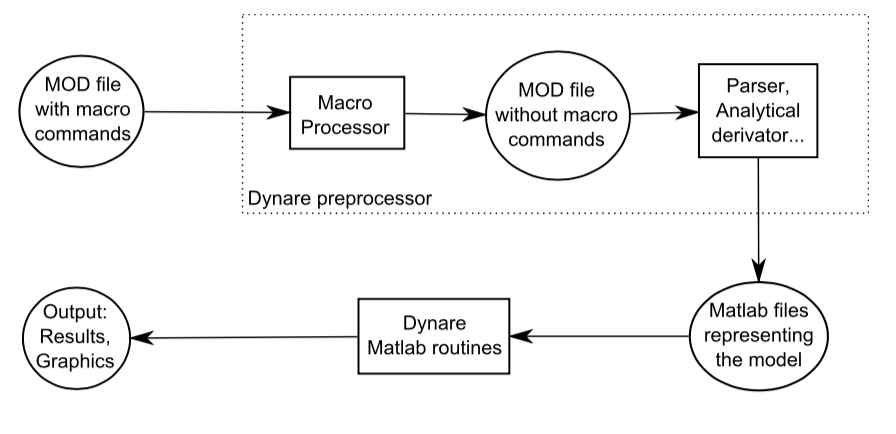
\includegraphics[width=10cm]{pictures/flowchart_macroprocessor}}
		\end{figure}
	\end{itemize}
\end{frame}
\subsubsection{Introduction to the Syntax}
\begin{frame}<presentation>
	\frametitle{{\thesection.\thesubsection.\thesubsubsection} Introduction to the Syntax (1)}
	\begin{itemize}
		\item The macro-processor is invoked by placing \textit{macro directives} in the .mod file. 
		\item Directives begin with: @\#  
		\item The main directives are:
		\begin{itemize}
			\item \texttt{@\#include}: file inclusion
			\item \texttt{@\#define}: definition of a macro processor variable
			\item \texttt{@\#if/@\#ifdef/@\#ifndef/@\#ifndef/@\#else/@\#endif}: conditional statements
			\item \texttt{@\#for/@\#endfor}: loop statements 
		\end{itemize}
	\item Most directives fit on one line. If needed however, two backslashes at the end of a line indicate that the directive is continued on the next line.
	\end{itemize}
\end{frame}
\begin{frame}<presentation>
	\frametitle{{\thesection.\thesubsection.\thesubsubsection} Introduction to the Syntax (2)}
	\begin{itemize}
		\item The macro processor has its own list of variables which are different than model variables and MATLAB/Octave variables.
		\item There are 4 types of macro-variables:
		\begin{itemize}
			\item integer
			\item string (declared between \textit{double} quotes)
			\item integer array
			\item string array
		\end{itemize}
		\item Note that there is no boolean type:
		\begin{itemize}
			\item false is represented by integer zero
			\item true is any non-zero integer
		\end{itemize} 
		\item Further note that, as the macro-processor cannot handle non-integer real numbers, integer division results in the quotient with the fractional part truncated (hence, $5/3=3/3=1$).
	\end{itemize}
\end{frame}
\begin{frame}<presentation>
	\frametitle{{\thesection.\thesubsection.\thesubsubsection} Introduction to the Syntax (3)}
	\begin{itemize}
		\justifying
		\item For a more comprehensive explanation of the syntax of the macro language, also containing illustrative examples, it is recommended to consider two following sources:
		\begin{itemize}
			\item S. Villemot and H. Bastani: The Dynare Macro Processor - Dynare Summer School 2019.
			\item Chapter 4.24 in Dynare: Reference Manual Version 4.
		\end{itemize}
	\end{itemize}
\end{frame}
\subsubsection{Common use}
\begin{frame}<presentation>
	\frametitle{{\thesection.\thesubsection.\thesubsubsection} Common use (1)}
	\begin{itemize}
		\item Add content.
	\end{itemize}
\end{frame}
\subsubsection{Example ?}

\section{DGE-CRED Model}

\subsection{Introduction}
\begin{frame}[plain]
\frametitle{Introduction}
\begin{itemize}
\item A dynamic general equilibrium model with optimizing agents
\item We differentiate between regions and economic activities.
\item Our model is implemented in the open source environment \href{https://www.dynare.org/}{Dynare} and can be run using Matlab or Octave.
\begin{itemize}
	\item Sectors in the model correspond to economic activities and the classification by the General Statistical Office (GSO).
	\item Regions are based on the statistical regions.
\end{itemize}
\item We extend the approach by \cite{nordhaus1993optimal} to model the impact of climate change through damage functions.
\end{itemize}
\end{frame}

\begin{frame}[plain]
\frametitle{Model Structure}
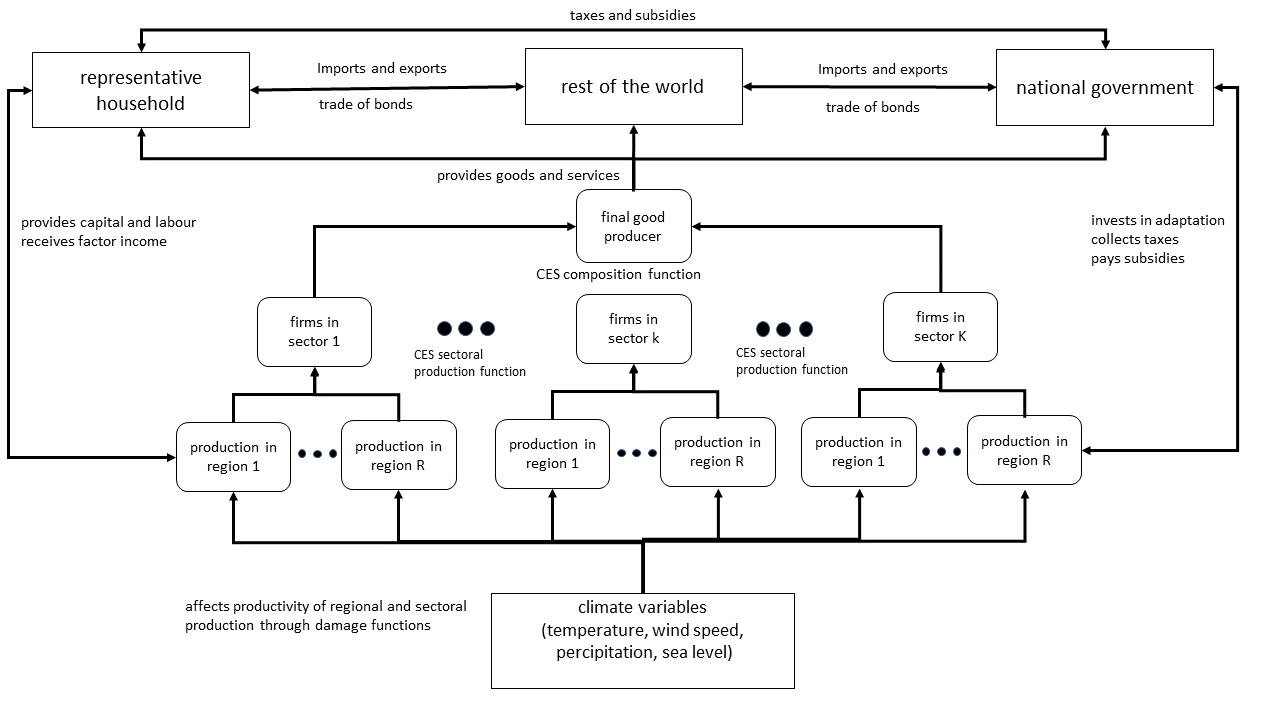
\includegraphics[width = 1\textwidth]{pictures/Model_Structure.png}
\end{frame}


\subsection{Demand}
\begin{frame}
\frametitle{Households}
\scriptsize
\begin{itemize}
\item representative households $h$ providing labour $N$ and capital $K$ to domestic firms $f$
\item maximize discounted utility over an infinite horizon by choosing consumption $C_t(h)$, capital $K_{k,r,t+1}(h)$, investments $I_{k,r,t}(h)$, labour $N_{k,r,t}(h)$ and foreign net wealth $B_{t+1}$
\item the optimization problem of the representative household is
\begin{align*}
 & \underset{C_t(h), \, K_{k,r,t+1}(h), \, I_{k,r,t}(h), , \, N_{k,r,t}(h), \, B_{t+1}}{\mbox{max}} \sum_{t=0}^{\infty} \beta^{t} \left(\frac{C_{t}(h)^{1 - \sigma^{C}}}{1 - \sigma^{C}} - \sum_{k=1}^{K} \sum_{r=1}^{R} A^{N}_{k,r,t} \, \phi^{L}_{k,r} \frac{N_{k,r,t}(h)^{1+\sigma^{L}}}{1+\sigma^{L}} \right) \\
\mbox{s.t.} & P_{t} \, C_{t}(h) \, (1 + \tau^{C}) + \sum_{k=1}^{K} \sum_{r=1}^{R} P_{k,r,t} I_{k,r,t}(h) + B_{t+1}(h) = \\
 & \sum_{k=1}^{K} \sum_{r=1}^{R} (1 - \tau^{N}) \, W_{k,r,t} N_{k,r,t}(h) + \sum_{k=1}^{K} \sum_{r=1}^{R} P_{k,r,t} \, r_{k,r,t} \, (1 - \tau^{K}) \, K_{k,r,t}(h) + S^{f}_{t} \, \phi^{B}_{t} \, (1 + r^{f}_{t} )\, B_{t}(h)
 %K_{k,r,t+1} = (1 - \delta - D^K_{k,r,t}) \, K_{k,r,t} - I_{k,r,t} \, \Gamma\left(\frac{I_{k,r,t}}{I_{k,r,t-1}}\right).
\end{align*}
\end{itemize}
\end{frame}


\begin{frame}
\frametitle{Households Lagrangian}
\scriptsize
\begin{itemize}
\item We set-up the Lagrangian for the optimization problem to derive the first order conditions.
\begin{align*}
& \sum_{t=0}^{\infty} \beta^{t} \Bigg[ \left(\frac{C_{t}(h)^{1 - \sigma^{C}}}{1 - \sigma^{C}} - \sum_{k=1}^{K} \sum_{r=1}^{R} A^{N}_{k,r,t} \, \phi^{L}_{k,r} \frac{N_{k,r,t}(h)^{1+\sigma^{L}}}{1+\sigma^{L}} \right) \\
& - \lambda_{t}(h) \Big(P_{t} \, C_{t}(h) \, (1 + \tau^{C}) + \sum_{k=1}^{K} \sum_{r=1}^{R} P_{k,r,t} I_{k,r,t}(h) + B_{t+1}(h) - \sum_{k=1}^{K} \sum_{r=1}^{R} (1 - \tau^{N}) \, W_{k,r,t} N_{k,r,t}(h) \\
& - \sum_{k=1}^{K} \sum_{r=1}^{R} P_{k,r,t} \, r_{k,r,t} \, (1 - \tau^{K}) \, K_{k,r,t}(h) - S^{f}_{t} \, \phi^{B}_{t} \, (1 + r^{f}_{t} )\, B_{t}(h) \Big) \\
& - \sum_{k=1}^{K} \sum_{r=1}^{R} \lambda_{t}(h) \omega^{I}_{k,r,t}(h) \left\lbrace K_{k,r,t+1} - (1 - \delta - D^K_{k,r,t}) \, K_{k,r,t} - I_{k,r,t} \, \Gamma\left(\frac{I_{k,r,t}}{I_{k,r,t-1}}\right) \right\rbrace\Bigg] .
\end{align*}
\end{itemize}
\end{frame}


\begin{frame}
\frametitle{Households First Order Conditions - Intratemporal}
\scriptsize
\begin{itemize}
\item Marginal utility of consumption
\begin{align*}
\lambda_{t} =\frac{C_{t}(h)^{-\sigma^{C}}}{P_{t}\, (1 + \tau^C)}
\end{align*}
\item Labour supply curve
\begin{align*}
\phi^{L}_{k,r} \, A^{N}_{k,r,t} \, N_{k,r,t}(h)^{\sigma^{L}} = \lambda_{t}(h) \, W_{k,r,t} \, (1 - \tau^{N}) \\
\end{align*}
\end{itemize}
\end{frame}


\begin{frame}
\frametitle{Households First Order Conditions - Intertemporal}
\scriptsize
\begin{itemize}
\item Euler equation for foreign bonds
\begin{align*}
\lambda_{t+1} \, \beta \, S^{f}_{t+1} \, \phi^{B}_{t+1} \left(1+{{r^{f}}_{t+1}}\right) = \lambda_{t} \\
\end{align*}
\item Euler equation for capital
\begin{align*}
\lambda_{t+1}(h) \, \beta \, \left(P_{k,r,t+1} \, r_{k,r,t+1} \, (1 - \tau^K) + (1 - \delta - D^{K}_{k,r,t+1}) \, \omega^{I}_{k,r,t+1} \right) = \lambda_{t}(h) \, \omega^{I}_{k,r,t}.
\end{align*}
\item Euler equation for investment
\begin{align*}
P_{k,r,t} \, \lambda_{t}(h) = \lambda_{t}(h) \, \omega^{I}_{k,r,t} \, \left(\Gamma(\frac{I_{k,r,t}}{I_{k,r,t-1}}) + \frac{\partial \Gamma(\frac{I_{k,r,t}}{I_{k,r,t-1}})}{\partial (\frac{I_{k,r,t}}{I_{k,r,t-1}})} \, \frac{I_{k,r,t}}{I_{k,r,t-1}} \right) - \beta \lambda_{t+1}(h) \, \omega^{I}_{k,r,t+1} \, \frac{\partial \Gamma(\frac{I_{k,r,t+1}}{I_{k,r,t}})}{\partial (\frac{I_{k,r,t+1}}{I_{k,r,t}})} \, \left(\frac{I_{k,r,t+1}}{I_{k,r,t}}\right)^2
\end{align*}
\item Investment adjustment cost
\begin{align*}
\Gamma(\frac{I_{k,r,t}}{I_{k,r,t-1}}) = 3 - exp\left\lbrace\sqrt{\phi^{K}/2}\left(\frac{I_{k,r,t}}{I_{k,r,t-1}}-1\right\rbrace\right) - exp\left\lbrace-\sqrt{\phi^{K}/2}\left(\frac{I_{k,r,t}}{I_{k,r,t-1}}-1\right)\right\rbrace
\end{align*}
\end{itemize}
\end{frame}

\begin{frame}
\frametitle{Households First Order Conditions - Intertemporal}
\scriptsize
\begin{itemize}
\item Euler equation for capital
\begin{align*}
\lambda_{t+1}(h) \, \beta \, \left(P_{k,r,t+1} \, r_{k,r,t+1} \, (1 - \tau^K) + (1 - \delta - D^{K}_{k,r,t+1}) \, \omega^{I}_{k,r,t+1} \right) = \lambda_{t}(h) \, \omega^{I}_{k,r,t}.
\end{align*}
\item Euler equation for investment
\begin{align*}
P_{k,r,t} \, \lambda_{t}(h) = \lambda_{t}(h) \, \omega^{I}_{k,r,t} \, \left(\Gamma(\frac{I_{k,r,t}}{I_{k,r,t-1}}) + \frac{\partial \Gamma(\frac{I_{k,r,t}}{I_{k,r,t-1}})}{\partial (\frac{I_{k,r,t}}{I_{k,r,t-1}})} \, \frac{I_{k,r,t}}{I_{k,r,t-1}} \right) - \beta \lambda_{t+1}(h) \, \omega^{I}_{k,r,t+1} \, \frac{\partial \Gamma(\frac{I_{k,r,t+1}}{I_{k,r,t}})}{\partial (\frac{I_{k,r,t+1}}{I_{k,r,t}})} \, \left(\frac{I_{k,r,t+1}}{I_{k,r,t}}\right)^2
\end{align*}
\end{itemize}
\end{frame}


\begin{frame}
\frametitle{Rest of the world}
\scriptsize
\begin{itemize}
\item Euler equation foreign bonds
\begin{align*}
\lambda_{t+1} \, \beta \, S^{f}_{t+1} \, \phi^{B}_{t+1} \left(1+{{r^{f}}_{t+1}}\right) = \lambda_{t}
\end{align*}
\item Effective exchange rate $S^f$ and the world interest rate $r^f$.
\item The required interest rate is above the world interest rate if the foreign debt ($B_{t+1}<0$)/ foreign claims ($B_{t+1}>0$) relative to GDP increases/decreases and future net exports relative to GDP will decrease. 
\begin{align*}
\phi^{B}_{t+1} = exp \left(-\phi^B \,(S^{f}_{t+1} \, r^{f}_{t+1} \, \frac{B_{t+1}}{Y_{t+1}}+\frac{NX_{t+1}}{Y_{t+1}})\right)
\end{align*}
\end{itemize}
\end{frame}


\begin{frame}
\frametitle{Government Budget Constraint}
\scriptsize
\begin{itemize}
\item We are interested in different policy measures taken by the government to adapt to a new climate regime. 
\item Government behaviour is not a result of an optimization problem. 
\begin{align*}
G_{t} + \sum_{k}^{K} \sum_{r}^{R} G^{A}_{k,r,t} + B^G_{t+1} =& \sum_{k}^{K} \sum_{r}^{R} \, \left\lbrace (\tau^{K} + \tau_{r,k,t}^{K}) \, P_{k,r,t} \, r_{k,r,t} \, K_{k,r,t} + (\tau^{N} + \tau_{k,r,t}^{N}) \, W_{k,r,t} \, N_{k,r,t} \, Pop_{t} \right\rbrace \nonumber \\
& + (1 + r^{f}_{t}) \, S^{f}_{t} \phi^{B}_{t} \, B^G_{t}
\end{align*}
\end{itemize}
\end{frame}

\begin{frame}
\frametitle{Government Policy Instruments}
\scriptsize
\begin{itemize}
\item Governments can invest into adaptation capital stocks
\begin{align*}
K^{A,z}_{k,r,t+1} = \eta^{A,z}_{k,r,t}
\end{align*}
\item Evolution of adaptation capital stocks
\begin{align*}
K^{A,z}_{k,r,t+1} = (1 - \delta_{K^{A,z},k,r}) \, K^{A,z}_{k,r,t} + G^{A,z}_{k,r,t} \nonumber \\
\end{align*}
\item Tax on capital expenditures paid by firms
\begin{align*}
\tau^{K}_{k,r,t} = \tau^{K}_{k,r,0} + \eta^{\tau^{K}}_{k,r,t} \nonumber \\
\end{align*}
\item Tax rate on wage bill paid by firms
\begin{align*}
\tau^{N}_{k,r,t} = \tau^{N}_{k,r,0} + \eta^{\tau^{N}}_{k,r,t} \nonumber \\
\end{align*}
\end{itemize}
\end{frame}

\begin{frame}
\frametitle{Resource constraint}
\scriptsize
\begin{itemize}
\item Households and government use domestic final goods $Y_t$ produced by firms for consumption, investment and for exports $X_{t}$ and can also use imports $M_t$ for consumption and investment
\begin{align}
Y_{t} = C_{t} + I_{t} + G_{t} + \underbrace{X_{t} - M_{t}}_{NX_{t}}
\end{align}
\item The aggregation of the budget constraints of the representative households also states that positive net exports are used to increase net financial wealth to the rest of the world.
\begin{align}
NX_t = B_{t+1} - (1 + r^{f}_{t}) S^{f}_{t} \phi^B_{t} B_{t}
\end{align}
\end{itemize}
\end{frame}

%
%
\subsection{Production}

\begin{frame}
\frametitle{Sectoral Decomposition}
\scriptsize
\begin{itemize}
\item Final domestic goods $Y_{t}$ are created combining goods from different sectors $Y_{k,t}$ using a CES production function.
\begin{align}
\underset{Y_{k,t}}{\mathrm{min}} & \sum_{k} Y_{k,t} \, P_{k,t} \\ 
Y_{t} &= \left(\sum_{k} {\omega^{Q}_{k}}^{\frac{1}{\eta^Q}} Y_{k,t}^{\frac{\eta^Q-1}{\eta^Q}} \right)^{\frac{\eta^Q}{\eta^Q-1}}
\end{align}

\item Therefore, the demand for sectoral products correspond to the first order conditions of the above optimization problem. 
\begin{align*}
\frac{P_{k,t}}{P_{t}} &= {\omega^{Q}_{k}}^{\frac{1}{\eta^Q}} \left(\frac{Y_{k,t}}{Y_{t}}\right)^{\frac{-1}{\eta^Q}}
\end{align*}
\end{itemize}
\end{frame}



\begin{frame}
\frametitle{Regional Decomposition}
\scriptsize
\begin{itemize}
\item In order to model regional economic activity we further decompose the production process on a regional level.
\begin{align*}
\underset{Y_{k,r,t}}{\mathrm{min}} & \sum_{k} Y_{k,r,t} \, P_{k,r,t} \\ 
Y_{k,t} &= \left(\sum_{k} {\omega^{Q}_{k,r}}^{\frac{1}{\eta^Q_{k}}} Y_{k,r,t}^{\frac{\eta^Q_{k}-1}{\eta^Q_{k}}} \right)^{\frac{\eta^Q_{k}}{\eta^Q_{k}-1}}
\end{align*}
\item Demand for sectoral and regional products correspond to the first order conditions of the above optimization problem.
\begin{align*}
\frac{P_{k,r,t}}{P_{k,t}} &= {\omega^{Q}_{k,r}}^{\frac{1}{\eta^{Q}_{k}}} \left(\frac{Y_{k,r,t}}{Y_{k,t}}\right)^{\frac{-1}{\eta^{Q}_{k}}}
\end{align*}
\end{itemize}
\end{frame}

\begin{frame}
\frametitle{Regional Production}
\scriptsize
\begin{itemize}
\item At the regional and sectoral level are representative firms maximizing profits using capital $K_{k,r,t}$ and labour $L_{k,r,t} = N_{k,r,t} \, Pop_{t}$ provided by households to produce products. 
\item They charge a price $P_{k,r,t}$ for their products and have to pay households wages $W_{k,r,t}$, interest on rented capital $P_{r,k,t} \, r_{r,k,t}$, taxes related to the wage bill $\tau^{N}_{r,k,t}$ and on capital expenditure $\tau^{K}_{r,k,t}$.
\item Representative firms have access to a regional and sector specific constant elasticity of substitution production function.
\item The productivity of capital and labour of a firm in one sector and region depends on the climate variables, and the adaption measures by the government represented by a damage function affecting total factor productivity $A_{k,r,t}$ by $D_{k,r,t} = D_{k,r}\left(T_{r,t}, \, PREC_{r,t}, \, WS_{r,t}, \, SL_{r,t}, \, CYC_{r,t}, \, DRO_{r,t}, \, G^{A}_{r,k,t} \right)$.
\item Further, we explicitly differentiate between climate induced damages affecting labour productivity $D_{N,k,r,t}$ and capital depreciation $D_{K,k,r,t}$. 
\item As in \cite{nordhaus1993optimal}, we assume a polynomial functional form of the damage functions, but the damages are different across regions and sectors.
\end{itemize}
\end{frame}


\begin{frame}
\frametitle{Damages on TFP}
\tiny
\begin{align*}
{{D_{k,r}}_{t}} &= \Big\lbrace \nonumber \\
 & (\underbrace{{{a_{T,1,k,r}}} \, {{T_{r}}_{t}}+{{a_{T,2,k,r}}}\, \left({T_{r}}_{t}\right)^{a_{T,3,k,r}}}_{\mbox{impact of temperature}})  \, \underbrace{exp(-\phi^{G^{A,T}}_{k,r} K^{A,T}_{k,r,t})}_{\mbox{impact of adaptation}} \, 
 + (\underbrace{{{a_{SL,1,k,r}}}\, {{SL}_{t}}+{{a_{SL,2,k,r}}}\, \left({SL}_{t}\right)^{{{a_{SL,3,k,r}}}}}_{\mbox{impact of sea level}})   \, \underbrace{I(SL > \frac{K^{A,SL}_{k,r,t}}{\phi^{G^{A,SL}}_{k,r}})}_{\mbox{impact of adaptation}} \\
& +  (\underbrace{{{a_{WS,1,k,r}}}\, {{WS_{r}}_{t}}+{{a_{WS,2,k,r}}}\, \left({WS_{r}}_{t}\right)^{{{a_{WS,3,k,r}}}}}_{\mbox{impact of wind speed}}) \, \underbrace{exp(-\phi^{G^{A,WS}}_{k,r} K^{A,WS}_{k,r,t})}_{\mbox{impact of adaptation}} \\
& + (\underbrace{{{a_{PREC,1,k,r}}} \, {{PREC_{r}}_{t}}+{{a_{PREC,2,k,r}}}\, \left({PREC_{r}}_{t}\right)^{{{a_{PREC,3,k,r}}}}}_{\mbox{impact of precipitation}}) \, \underbrace{exp(-\phi^{G^{A,PREC}}_{k,r} K^{A,PREC}_{k,r,t})}_{\mbox{impact of adaptation}} \nonumber \\
& +  (\underbrace{{{a_{CYC,1,k,r}}}\, {{CYC_{r}}_{t}}+{{a_{CYC,2,k,r}}}\, \left({CYC_{r}}_{t}\right)^{{{a_{CYC,3,k,r}}}}}_{\mbox{impact of cyclones}}) \, \underbrace{exp(-\phi^{G^{A,CYC}}_{k,r} K^{A,CYC}_{k,r,t})}_{\mbox{impact of adaptation}} \\
& +  (\underbrace{{{a_{DRO,1,k,r}}} \, {{DRO_{r}}_{t}}+{{a_{DRO,2,k,r}}}\, \left({DRO_{r}}_{t}\right)^{{{a_{DRO,3,k,r}}}}}_{\mbox{impact of droughts}}) \, \underbrace{exp(-\phi^{G^{A,DRO}}_{k,r} K^{A,DRO}_{k,r,t})}_{\mbox{impact of adaptation}} \\
& \Big\rbrace.
\end{align*}
\end{frame}

\begin{frame}
\frametitle{Damages on Labour Productivity}
\tiny
\begin{align*}
{{D^{N}_{k,r}}_{t}}=& \Big( \nonumber \\
&\underbrace{{{a^{N}_{T,1,k,r}}} \, {{T_{r}}_{t}}+{{a^{N}_{T,2,k,r}}}\, \left({T_{r}}_{t}\right)^{a^{N}_{T,3,k,r}}}_{\mbox{impact of temperature}} + 
\underbrace{{{a^{N}_{SL,1,k,r}}}\, {{SL}_{t}}+{{a^{N}_{SL,2,k,r}}}\, \left({SL}_{t}\right)^{{{a^{N}_{SL,3,k,r}}}}}_{\mbox{impact of sea level}} \nonumber \\
+ & \underbrace{{{a^{N}_{WS,1,k,r}}}\, {{WS_{r}}_{t}}+{{a^{N}_{WS,2,k,r}}}\, \left({WS_{r}}_{t}\right)^{{{a^{N}_{WS,3,k,r}}}}}_{\mbox{impact of wind speed}} 
+ (\underbrace{{{a^{N}_{PREC,1,k,r}}} \, {{PREC_{r}}_{t}}+{{a^{N}_{PREC,2,k,r}}}\, \left({PREC_{r}}_{t}\right)^{{{a^{N}_{PREC,3,k,r}}}}}_{\mbox{impact of precipitation}}) \,  \nonumber \\
+ & \underbrace{{{a^{N}_{CYC,1,k,r}}}\, {{CYC_{r}}_{t}}+{{a^{N}_{CYC,2,k,r}}}\, \left({CYC_{r}}_{t}\right)^{{{a^{N}_{CYC,3,k,r}}}}}_{\mbox{impact of cyclones}}
+ \underbrace{{{a^{N}_{DRO,1,k,r}}} \, {{DRO_{r}}_{t}}+{{a^{N}_{DRO,2,k,r}}}\, \left({DRO_{r}}_{t}\right)^{{{a^{N}_{DRO,3,k,r}}}}}_{\mbox{impact of droughts}} \nonumber \\
&\Big).
\end{align*}
\end{frame}

\begin{frame}
\frametitle{Damages on Capital}
\tiny
\begin{align*}
{{D^{K}_{k,r}}_{t}}=& \Big( \nonumber \\
&\underbrace{{{a^{K}_{T,1,k,r}}} \, {{T_{r}}_{t}}+{{a^{K}_{T,2,k,r}}}\, \left({T_{r}}_{t}\right)^{a^{K}_{T,3,k,r}}}_{\mbox{impact of temperature}}+ \underbrace{{{a^{K}_{SL,1,k,r}}}\, {{SL}_{t}}+{{a^{K}_{SL,2,k,r}}}\, \left({SL}_{t}\right)^{{{a^{K}_{SL,3,k,r}}}}}_{\mbox{impact of sea level}} \nonumber \\
+ & \underbrace{{{a^{K}_{WS,1,k,r}}}\, {{WS_{r}}_{t}}+{{a^{K}_{WS,2,k,r}}}\, \left({WS_{r}}_{t}\right)^{{{a^{K}_{WS,3,k,r}}}}}_{\mbox{impact of wind speed}}
+ \underbrace{{{a^{K}_{PREC,1,k,r}}} \, {{PREC_{r}}_{t}}+{{a^{K}_{PREC,2,k,r}}}\, \left({PREC_{r}}_{t}\right)^{{{a^{K}_{PREC,3,k,r}}}}}_{\mbox{impact of precipitation}} \nonumber \\
+ & \underbrace{{{a^{K}_{CYC,1,k,r}}}\, {{CYC_{r}}_{t}}+{{a^{K}_{CYC,2,k,r}}}\, \left({CYC_{r}}_{t}\right)^{{{a^{K}_{CYC,3,k,r}}}}}_{\mbox{impact of cyclones}}
+ \underbrace{{{a^{K}_{DRO,1,k,r}}} \, {{DRO_{r}}_{t}}+{{a^{K}_{DRO,2,k,r}}}\, \left({DRO_{r}}_{t}\right)^{{{a^{K}_{DRO,3,k,r}}}}}_{\mbox{impact of droughts}} \nonumber \\
&\Big).
\end{align*}
\end{frame}


\begin{frame}
\frametitle{Profit Maximization}
\scriptsize
\begin{itemize}
\item Firms in each region and sector have access to a constant elasticity of substitution production function with production factors labour and capital.
\begin{align*}
\underset{Y_{k,r,t}, N_{k,r,t}, K_{k,r,t}}{\mathrm{max}} P_{k,r,t} \, Y_{k,r,t} - W_{k,r,t} \, N_{k,r,t} \, Pop_{t} \, (1 + \tau^{N}_{k,r,t}) - r_{k,r,t} \, P_{k,r,t} \, K_{k,r,t} \, (1 + \tau^{K}_{k,r,t})\nonumber \\ 
\mbox{s.t.} \, Y_{k,r,t} = A_{k,r,t} (1 - D_{k,r,t}) \, \left[{\alpha^{N}_{k,r}}^{\frac{1}{\eta^{NK}_{k,r}}} \, \left( A^{N}_{k,r,t} \, (1 - D^{N}_{k,r,t}) \, Pop_{t} \, N_{k,r,t}\right)^{\rho_{k,r}} + {\alpha^{K}_{k,r}}^{\frac{1}{\eta^{NK}_{k,r}}} \, \left(K_{k,r,t}\right)^{\rho_{k,r}}\right]^{\frac{1}{\rho_{k,r}}}, \nonumber \\
\mbox{ where } \rho_{k,r} = \frac{\eta^{NK}_{k} - 1}{\eta^{NK}_{k}}.
\end{align*}
\end{itemize}
\end{frame}


\begin{frame}
\frametitle{Factor Demand}
\scriptsize
\begin{itemize}
\item Demand for production factors are given by the first order condition of the above optimization problem. The Lagrange multiplier is equal to the price charged by companies. 
\begin{align*}
\frac{W_{k,r,t}}{P_{k,r,t}}  \, (1 + \tau^{N}_{k,r,t}) = {\alpha^{N}_{k,r}}^{\frac{1}{\eta^{NK}_{k,r}}} \, \left(A_{k,r,t} \, (1 - D_{k,r,t}) \, A^N_{k,r,t} \, (1 - D^N_{k,r,t})\right)^{\rho_{k,r}} \left(\frac{Pop_{t} N_{k,r,t}}{Y_{k,r,t}}\right)^{-\frac{1}{\eta^{NK}_{k,r}}} \nonumber \\ 
r_{k,r,t} \, (1 + \tau^{K}_{k,r,t}) = {\alpha^{K}_{k,r}}^{\frac{1}{\eta^{NK}_{k,r}}} \, \left(A_{k,r,t} \, (1 - D_{k,r,t})\right)^{\rho_{k,r}}\left(\frac{K_{k,r,t}}{Y_{k,r,t}} \right)^{-\frac{1}{\eta^{NK}_{k,r}}} \\ 
\end{align*}
\item We use the more general case of the CES production function rather than the more commonly used Cobb-Douglas production function. 
\item The parameter $\eta^{NK}_{k,r}$ allows us to control the response of capital and labour demand to temporary productivity shocks. 
\item Temporary productivity shocks are in our set-up also weather extremes. 
\end{itemize}
\end{frame}

\begin{frame}
\frametitle{Trade with the rest of the world}
\scriptsize
\begin{itemize}
\item The demand for domestic exports and foreign imports is not explicitly modeled in this version of the model. 
\item We assume that net exports follow an auto-regressive process of order one and that the long-run value of net exports depend on the long-run development of gross domestic product.
\begin{align*}
NX_{t} = \rho^{NX} \, NX_{t-1} + (1 - \rho^{NX}) \omega^{NX} P_{t} \, Y_{t} \, exp\left({{\eta_{NX}}_{t}}\right)
\end{align*}
\item The effective exchange rate $S^f_{t}$ and the world interest rate $r^{f}_{t}$ determine how much governments and households have to pay back in domestic currency as net lender or how much they receive as net borrower to the rest of the world. \item Here the world interest rate is independent of domestic developments and only the effective exchange rate adjusts.
\end{itemize}
\end{frame}

\section{Model Simulation and Calibration}

\begin{frame}[allowframebreaks]%in case more than 1 slide needed
\frametitle{References}
\scriptsize{
\printbibliography}
\end{frame}

\end{document}
